% Created by tikzDevice version 0.12.3.1 on 2021-07-09 13:56:00
% !TEX encoding = UTF-8 Unicode
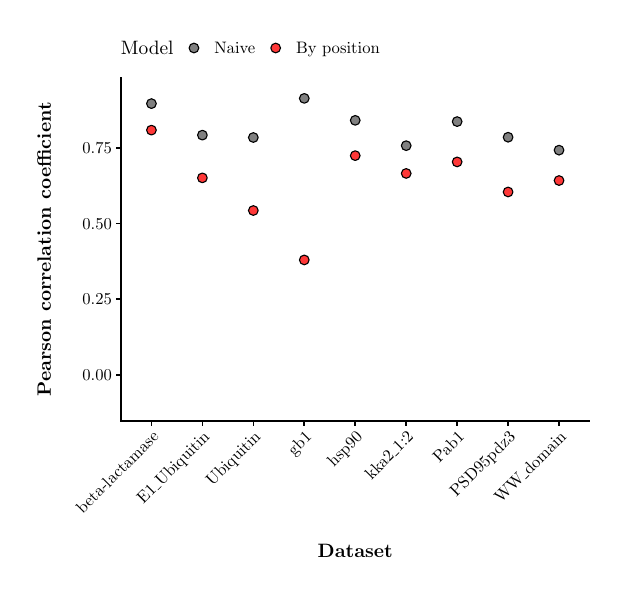
\begin{tikzpicture}[x=1pt,y=1pt]
	\definecolor{fillColor}{RGB}{255,255,255}
	\path[use as bounding box,fill=fillColor,fill opacity=0.00] (0,0) rectangle (206.56,196.49);
	\begin{scope}
		\path[clip] ( 33.67, 54.47) rectangle (203.06,178.29);
		\definecolor{drawColor}{RGB}{0,0,0}
		\definecolor{fillColor}{RGB}{128,128,128}

		\path[draw=drawColor,line width= 0.4pt,line join=round,line cap=round,fill=fillColor] ( 63.13,157.66) circle (  1.75);

		\path[draw=drawColor,line width= 0.4pt,line join=round,line cap=round,fill=fillColor] (173.60,156.90) circle (  1.75);

		\path[draw=drawColor,line width= 0.4pt,line join=round,line cap=round,fill=fillColor] (155.19,162.55) circle (  1.75);

		\path[draw=drawColor,line width= 0.4pt,line join=round,line cap=round,fill=fillColor] ( 81.54,156.80) circle (  1.75);

		\path[draw=drawColor,line width= 0.4pt,line join=round,line cap=round,fill=fillColor] (192.01,152.23) circle (  1.75);

		\path[draw=drawColor,line width= 0.4pt,line join=round,line cap=round,fill=fillColor] ( 44.72,169.05) circle (  1.75);

		\path[draw=drawColor,line width= 0.4pt,line join=round,line cap=round,fill=fillColor] ( 99.95,170.94) circle (  1.75);

		\path[draw=drawColor,line width= 0.4pt,line join=round,line cap=round,fill=fillColor] (118.36,163.00) circle (  1.75);

		\path[draw=drawColor,line width= 0.4pt,line join=round,line cap=round,fill=fillColor] (136.78,153.85) circle (  1.75);

		\visible<2->{%
			\definecolor{fillColor}{RGB}{255,56,56}

			\path[draw=drawColor,line width= 0.4pt,line join=round,line cap=round,fill=fillColor] ( 63.13,142.21) circle (  1.75);

			\path[draw=drawColor,line width= 0.4pt,line join=round,line cap=round,fill=fillColor] (173.60,137.12) circle (  1.75);

			\path[draw=drawColor,line width= 0.4pt,line join=round,line cap=round,fill=fillColor] (155.19,147.98) circle (  1.75);

			\path[draw=drawColor,line width= 0.4pt,line join=round,line cap=round,fill=fillColor] ( 81.54,130.42) circle (  1.75);

			\path[draw=drawColor,line width= 0.4pt,line join=round,line cap=round,fill=fillColor] (192.01,141.25) circle (  1.75);

			\path[draw=drawColor,line width= 0.4pt,line join=round,line cap=round,fill=fillColor] ( 44.72,159.47) circle (  1.75);

			\path[draw=drawColor,line width= 0.4pt,line join=round,line cap=round,fill=fillColor] ( 99.95,112.56) circle (  1.75);

			\path[draw=drawColor,line width= 0.4pt,line join=round,line cap=round,fill=fillColor] (118.36,150.25) circle (  1.75);

			\path[draw=drawColor,line width= 0.4pt,line join=round,line cap=round,fill=fillColor] (136.78,143.82) circle (  1.75);
		}%
	\end{scope}
	\begin{scope}
		\path[clip] (  0.00,  0.00) rectangle (206.56,196.49);
		\definecolor{drawColor}{RGB}{0,0,0}

		\path[draw=drawColor,line width= 0.6pt,line join=round,line cap=rect] ( 33.67, 54.47) --
		( 33.67,178.29);
	\end{scope}
	\begin{scope}
		\path[clip] (  0.00,  0.00) rectangle (206.56,196.49);
		\definecolor{drawColor}{RGB}{0,0,0}

		\node[text=drawColor,anchor=base east,inner sep=0pt, outer sep=0pt, scale=  0.60] at ( 30.42, 68.96) {0.00};

		\node[text=drawColor,anchor=base east,inner sep=0pt, outer sep=0pt, scale=  0.60] at ( 30.42, 96.28) {0.25};

		\node[text=drawColor,anchor=base east,inner sep=0pt, outer sep=0pt, scale=  0.60] at ( 30.42,123.60) {0.50};

		\node[text=drawColor,anchor=base east,inner sep=0pt, outer sep=0pt, scale=  0.60] at ( 30.42,150.92) {0.75};
	\end{scope}
	\begin{scope}
		\path[clip] (  0.00,  0.00) rectangle (206.56,196.49);
		\definecolor{drawColor}{RGB}{0,0,0}

		\path[draw=drawColor,line width= 0.6pt,line join=round] ( 31.92, 71.03) --
		( 33.67, 71.03);

		\path[draw=drawColor,line width= 0.6pt,line join=round] ( 31.92, 98.35) --
		( 33.67, 98.35);

		\path[draw=drawColor,line width= 0.6pt,line join=round] ( 31.92,125.67) --
		( 33.67,125.67);

		\path[draw=drawColor,line width= 0.6pt,line join=round] ( 31.92,152.99) --
		( 33.67,152.99);
	\end{scope}
	\begin{scope}
		\path[clip] (  0.00,  0.00) rectangle (206.56,196.49);
		\definecolor{drawColor}{RGB}{0,0,0}

		\path[draw=drawColor,line width= 0.6pt,line join=round,line cap=rect] ( 33.67, 54.47) --
		(203.06, 54.47);
	\end{scope}
	\begin{scope}
		\path[clip] (  0.00,  0.00) rectangle (206.56,196.49);
		\definecolor{drawColor}{RGB}{0,0,0}

		\path[draw=drawColor,line width= 0.6pt,line join=round] ( 44.72, 52.72) --
		( 44.72, 54.47);

		\path[draw=drawColor,line width= 0.6pt,line join=round] ( 63.13, 52.72) --
		( 63.13, 54.47);

		\path[draw=drawColor,line width= 0.6pt,line join=round] ( 81.54, 52.72) --
		( 81.54, 54.47);

		\path[draw=drawColor,line width= 0.6pt,line join=round] ( 99.95, 52.72) --
		( 99.95, 54.47);

		\path[draw=drawColor,line width= 0.6pt,line join=round] (118.36, 52.72) --
		(118.36, 54.47);

		\path[draw=drawColor,line width= 0.6pt,line join=round] (136.78, 52.72) --
		(136.78, 54.47);

		\path[draw=drawColor,line width= 0.6pt,line join=round] (155.19, 52.72) --
		(155.19, 54.47);

		\path[draw=drawColor,line width= 0.6pt,line join=round] (173.60, 52.72) --
		(173.60, 54.47);

		\path[draw=drawColor,line width= 0.6pt,line join=round] (192.01, 52.72) --
		(192.01, 54.47);
	\end{scope}
	\begin{scope}
		\path[clip] (  0.00,  0.00) rectangle (206.56,196.49);
		\definecolor{drawColor}{RGB}{0,0,0}

		\node[text=drawColor,rotate= 45.00,anchor=base east,inner sep=0pt, outer sep=0pt, scale=  0.60] at ( 47.64, 48.30) {beta-lactamase};

		\node[text=drawColor,rotate= 45.00,anchor=base east,inner sep=0pt, outer sep=0pt, scale=  0.60] at ( 66.05, 48.30) {E1\_Ubiquitin};

		\node[text=drawColor,rotate= 45.00,anchor=base east,inner sep=0pt, outer sep=0pt, scale=  0.60] at ( 84.46, 48.30) {Ubiquitin};

		\node[text=drawColor,rotate= 45.00,anchor=base east,inner sep=0pt, outer sep=0pt, scale=  0.60] at (102.88, 48.30) {gb1};

		\node[text=drawColor,rotate= 45.00,anchor=base east,inner sep=0pt, outer sep=0pt, scale=  0.60] at (121.29, 48.30) {hsp90};

		\node[text=drawColor,rotate= 45.00,anchor=base east,inner sep=0pt, outer sep=0pt, scale=  0.60] at (139.70, 48.30) {kka2\_1:2};

		\node[text=drawColor,rotate= 45.00,anchor=base east,inner sep=0pt, outer sep=0pt, scale=  0.60] at (158.11, 48.30) {Pab1};

		\node[text=drawColor,rotate= 45.00,anchor=base east,inner sep=0pt, outer sep=0pt, scale=  0.60] at (176.52, 48.30) {PSD95pdz3};

		\node[text=drawColor,rotate= 45.00,anchor=base east,inner sep=0pt, outer sep=0pt, scale=  0.60] at (194.93, 48.30) {WW\_domain};
	\end{scope}
	\begin{scope}
		\path[clip] (  0.00,  0.00) rectangle (206.56,196.49);
		\definecolor{drawColor}{RGB}{0,0,0}

		\node[text=drawColor,anchor=base,inner sep=0pt, outer sep=0pt, scale=  0.70] at (118.36,  4.86) {\bfseries Dataset};
	\end{scope}
	\begin{scope}
		\path[clip] (  0.00,  0.00) rectangle (206.56,196.49);
		\definecolor{drawColor}{RGB}{0,0,0}

		\node[text=drawColor,rotate= 90.00,anchor=base,inner sep=0pt, outer sep=0pt, scale=  0.70] at (  8.39,116.38) {\bfseries Pearson correlation coefficient};
	\end{scope}
	\begin{scope}
		\path[clip] (  0.00,  0.00) rectangle (206.56,196.49);
		\definecolor{drawColor}{RGB}{0,0,0}

		\node[text=drawColor,anchor=base west,inner sep=0pt, outer sep=0pt, scale=  0.70] at ( 33.67,186.73) {Model};
	\end{scope}
	\begin{scope}
		\path[clip] (  0.00,  0.00) rectangle (206.56,196.49);
		\definecolor{drawColor}{RGB}{0,0,0}
		\definecolor{fillColor}{RGB}{128,128,128}

		\path[draw=drawColor,line width= 0.4pt,line join=round,line cap=round,fill=fillColor] ( 60.08,189.14) circle (  1.75);
	\end{scope}
	\visible<2->{%
		\begin{scope}
			\path[clip] (  0.00,  0.00) rectangle (206.56,196.49);
			\definecolor{drawColor}{RGB}{0,0,0}
			\definecolor{fillColor}{RGB}{255,56,56}

			\path[draw=drawColor,line width= 0.4pt,line join=round,line cap=round,fill=fillColor] ( 89.61,189.14) circle (  1.75);
		\end{scope}
	}%
	\begin{scope}
		\path[clip] (  0.00,  0.00) rectangle (206.56,196.49);
		\definecolor{drawColor}{RGB}{0,0,0}

		\node[text=drawColor,anchor=base west,inner sep=0pt, outer sep=0pt, scale=  0.60] at ( 67.43,187.07) {Naive};
	\end{scope}
	\visible<2->{%
		\begin{scope}
			\path[clip] (  0.00,  0.00) rectangle (206.56,196.49);
			\definecolor{drawColor}{RGB}{0,0,0}

			\node[text=drawColor,anchor=base west,inner sep=0pt, outer sep=0pt, scale=  0.60] at ( 96.96,187.07) {By position};
		\end{scope}
	}%
\end{tikzpicture}
